\section{Modify User}
Modify User allows users to change certain values in the user's data by providing the user name. Users can change their username, height, goal, password, and gender.

\subsection*{Parameters}
\begin{description}
    \item [userID] The \texttt{UiD} of the user to who's statistics that will be modified. If this is not provided, there is no way of changing the user.
    \item [newUsername] The new username property of the user. If this statistic will not change, pass a \texttt{'0'} to the function. Otherwise, proceed with changing.
    \item [newHeightFeet] See above.
    \item [newHeightInches] See above.
    \item [newGoal] See above.
    \item [newPassword] See above.
    \item [newGender] See above.
\end{description}

\subsection*{Results}
For all attributes that do not have the value of \texttt{'0'}, the value of said attribute will be updated (provided it upholds all constraint).

\begin{center}
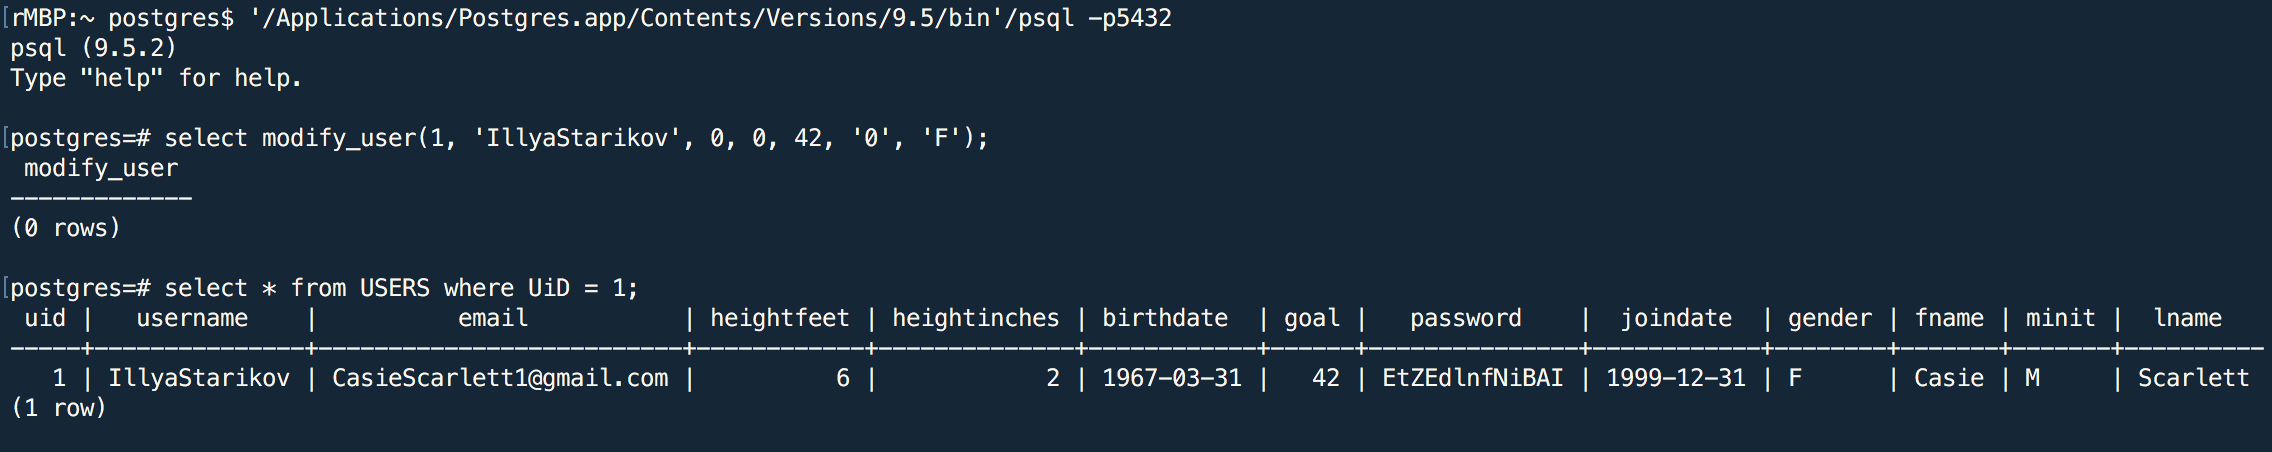
\includegraphics[width=\columnwidth]{include/assets/screenshots/modify_user}
\end{center}